El objetivo de la plan de gestión de riesgos es identificar, analizar y planificar la respuesta a los distintos riesgos a los que está expuesto el proyecto, de esta manera se busca minimizar la probabilidad de ocurrencia de los riesgos y reducir el impacto de los mismos en el proyecto.
\subsection*{Metodología aplicada}
Este plan se ha realizado siguiendo principalmente la metodología Boehm \cite{boehm1991} que divide la gestión de riesgos en dos fases: valoración de riesgos y control de riesgos. Cabe destacar que esta metodología ha sido adaptada a las necesidades del proyecto, añadiendo el paso previo de planificación según la metodología PMBOK \cite{pmbok2013}. De esta manera, finalmente tenemos tres fases:

\begin{itemize}
    \item \textbf{Planificar la gestión de riesgos:} Definir los objetivos, alcance, metodología y responsabilidades.
    \item \textbf{Valoración de riesgos:} Identificar, analizar y priorizar los riesgos.
    \item \textbf{Control de riesgos:} Planificar las respuestas, resolver y monitorear los riesgos.
\end{itemize}

\subsection*{Planificación de la gestión de riesgos}
\subsubsection*{Categorías de riesgos}
Basánsose en la estructura de desglose de riesgo representadas en el PMBOK, se han identificado las siguientes categorías de riesgos para el proyecto:

\begin{figure}[H]
    \hypertarget{fig:A1_PGR_RBS}{}
    \centering
    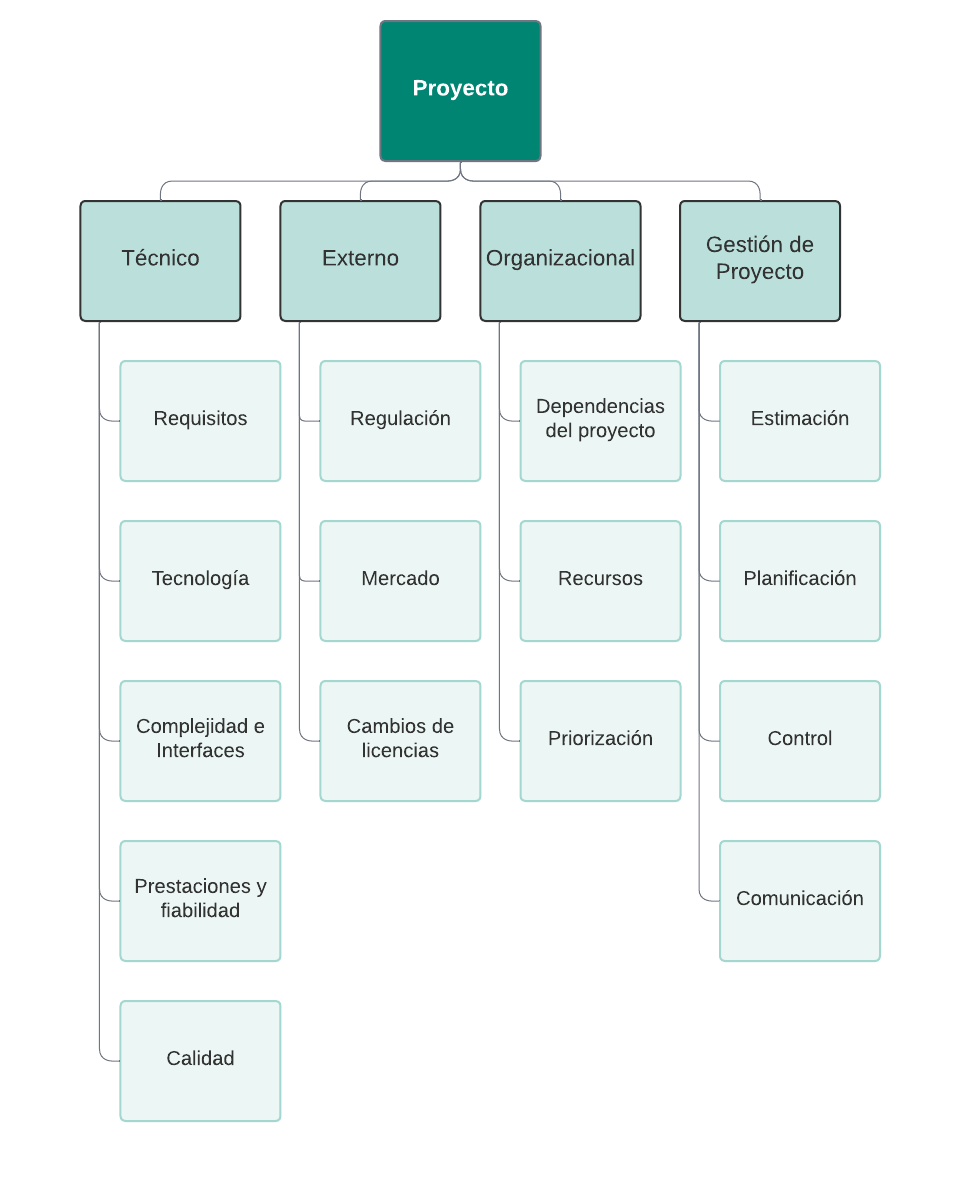
\includegraphics[width=0.65\linewidth]{figures/A1_PGR_RBS.png}
    \caption{RBS, desglose de categorías de riesgos del proyecto}
    \label{fig:A1_PGR_RBS}
\end{figure}

\subsubsection*{Probabilidad e impacto}
Para la valoración de riesgos se ha utilizado la \coloredUnderline{\hyperlink{fig:A1_PGR_matriz_prob_vs_impact}{matriz de probabilidad vs impacto}} definida anteriormente. 
Esta matriz establece los valores utilizados en la priorización de riesgos. Cada riesgo tiene un valor asociado de acuerdo a su probabilidad de ocurrencia y el impacto en el proyecto.

\begin{figure}[H]
    \hypertarget{fig:A1_PGR_matriz_prob_vs_impact}{}
    \centering
    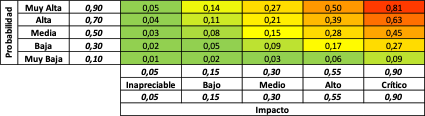
\includegraphics{figures/A1_PGR_matriz_prob_vs_impact.png}
    \caption{Matriz de probabilidad vs impacto}
    \label{fig:A1_PGR_matriz_prob_vs_impact}
\end{figure}

\subsubsection*{Identificación de riesgos}
Para la identificación de riesgos se han utilizado dos técnicas principales: la recopilación de información mediante \textit{brainstorming} y, de forma complementaria, el análisis de listas de control. La combinación de estas técnicas ha permitido una identificación de riesgos realista, abarcando tanto los riesgos inherentes al tipo de proyecto, es decir, desarrollo de software, como los riesgos específicos del proyecto en particular.

\subsubsection*{Análisis de riesgos}
Una vez identificados los riesgos, se ha procedido a analizarlos. Se ha llevado a cabo un análisis cualitativo de los riesgos que consta de los siguientes procesos:
\begin{itemize}
    \item \textbf{Evaluación de la probabilidad e impacto:} Asignación de valores de probabilidad e impacto a cada riesgo, obteniendo un valor de prioridad basado en la \coloredUnderline{\hyperlink{fig:A1_PGR_matriz_prob_vs_impact}{matriz de probabilidad vs impacto}}.
    \item \textbf{Categorización de riesgos:} Clasificación de los riesgos según las \coloredUnderline{\hyperlink{fig:A1_PGR_RBS}{categorías de riesgos}} identificadas.
    \item \textbf{Evaluación de la urgencia:} Priorización preliminar de los riesgos basada en la urgencia con la que deben ser tratados.
\end{itemize}
